\documentclass[11pt]{article}
\usepackage{graphicx}
\usepackage[margin=2.5cm]{geometry}
\usepackage{tikz}
\usepackage{indentfirst}
\usepackage{tabularx}
\usepackage{listingsutf8}
\usepackage{color}
\usepackage{titlesec}
\usepackage[portuguese]{babel}

\setcounter{secnumdepth}{4}

\graphicspath{{./images/}}

\def\checkmark{\tikz\fill[scale=0.4](0,.35) -- (.25,0) -- (1,.7) -- (.25,.15) -- cycle;} 
\setlength{\parskip}{0.5em}

\lstset{
	belowcaptionskip=1\baselineskip,
	captionpos=b,
	frame=tb,
	language=C,
	aboveskip=3mm,
	belowskip=3mm,
	showstringspaces=false,
	columns=flexible,
	basicstyle={\small\ttfamily},
	numbers=none,
	numberstyle=\tiny\color{gray},
	keywordstyle=\color{blue},
	commentstyle=\color{dkgreen},
	stringstyle=\color{mauve},
	breaklines=true,
	breakatwhitespace=true,
	tabsize=3,
	inputencoding=utf8,
	extendedchars=true,
	literate={á}{{\'a}}1 {ã}{{\~a}}1 {à}{{\`a} }1 {Ã}{{\~A}}1 {ó}{{\'o}}1 {Ó}{{\'O}}1 {Í}{{\'I}}1 {í}{{\'i}}1 {é}{{\'e}}1 {ç}{{\c{c}}}1 {Ç}{{\c{C}}}1 {ú}{{\'u}}1
}

\begin{document}
	\begin{titlepage}
	\begin{center}
		
		
\includegraphics[width=0.3\textwidth]{logo-isec}
		
		\normalsize
		Licenciatura em Engenharia Informática - Curso Europeu \\
		28 de maio de 2021
		
		\LARGE
		Gestão - 2020/2021
		
		\large
		Doutor Jorge Alexandre Almeida
		
		\vspace{1.5cm}
		
		
\includegraphics[width=0.3\textwidth]{logo}

		\vspace{0.5cm}

		\Huge
		\textbf{AquiTerrenos, Lda}
		
		\LARGE
		\textbf{Plano de Negócios}
		
		\vspace*{\fill}
		
		\Large
		
		\begin{tabular}{ccc}
			\textbf{Sofia Janeiro} & \textbf{José Almeida} & \textbf{Rúben Lousada} \\ 
			2019132578 & 2019129077 & 2019126176 \\
		\end{tabular}
	
		\vspace{.5cm}
		
		\vfill
		\vspace*{\fill}
		
		
	\end{center}
\end{titlepage}
	
	\tableofcontents
	\pagebreak
	
	\large
	\section{Sumário Executivo}
	
	\normalsize
	
	Possuir e manter terrenos é algo que faz parte da vida de muitos indivíduos e famílias. Por vezes, por falta de visão geral e/ou de conhecimento acerca dos próprios terrenos que possuem, podem-se gerar desentendimentos e dificuldades na sua localização. Com o crescimento da literacia informática da população, faz todo o sentido a procura da informatização do seu património. Muitas vezes, os proprietários dos terrenos procuram fazê-lo, mas não encontram uma solução viável e simples.
	
	A AquiTerrenos pretende resolver esse problema: tem como finalidade servir como uma pequena base de dados para cada família ou indivíduo, onde pode guardar toda a informação que achar relevante sobre os seus terrenos (como pinhais, eucaliptais, vinhas, etc.), assim como partilhar o acesso à mesma com quem quiser, facilitando o acesso a outros serviços externos.
	
	O nosso objetivo é dar ao cliente uma visão alargada sobre os seus terrenos, que o permita gerir os mesmos da forma mais eficiente possível, assim como partilhar informações dos mesmos à sua família / amigos / cooperativas agrícolas, de modo a fomentar e facilitar a cooperação entre proprietários. Implementaremos funcionalidades como geolocalização, informações topográficas, do solo, da fauna e da flora, visualização 3D e 360ª do terreno, entre outras.
	
	Para tirar o máximo proveito dessas funcionalidades, a AquiTerrenos funcionará também como um mercado de terrenos, que irá usar as informações já inseridas pelo cliente sobre os seus terrenos, caso este queira vender os mesmos. Isto simplifica o processo de venda para utilizadores da funcionalidade descrita nos parágrafos anteriores, pois, num caso ideal, já não será necessária a inserção de informação adicional sobre os terrenos que pretende vender, algo que fará com que o utilizador seja mais propício a usar o mercado da AquiTerrenos, e não qualquer outro.
	
	Esta proposta de solução tem de ser rentável para a empresa. Assim, surge a ideia de criação de uma aplicação, inicialmente grátis, onde possa ser feita essa gestão dos terrenos, assim como interagir com o mercado. Algumas funcionalidades estarão barradas por um pagamento único, outras estarão associadas a subscrições mensais/anuais.
	
	A partir de um pequeno estudo de mercado, observamos que por volta de 25\% das famílias que participaram desse estudo não possuem um registo (em papel ou informatizado) dos terrenos que possuem. Este seria o público-alvo do nosso serviço. Além disso, 90\% reportou interesse em utilizar a nossa aplicação e o mercado associado.
	
	De momento, a empresa encontra-se num estado teórico, sendo o próximo passo o desenvolvimento de um protótipo de modo a estudar ainda mais o mercado e o nosso público alvo. Estimamos que, no fim de um período de 5 anos, teremos um VAL de 1.700.000€, assim como uma TIR de aproximadamente 116\%. Estimamos, também, a recuperação do investimento inicial em 4 anos.
	
	\pagebreak
	
	\large
	\section{Apresentação do Negócio}
	\subsection{Identificação da Empresa}
	
	\normalsize
	
	\begin{center}
		\begin{tabular}{ | l | r | }
			\hline
			Designação Social: & AquiTerrenos, Lda \\
			\hline
			Nº de Contribuinte: & 001122334 \\
			\hline 
			Distrito: & Coimbra \\
			\hline   
			Concelho: & Coimbra \\
			\hline   
			Localidade: & Coimbra \\
			\hline   
			Morada (Sede Social): & Rua Pedro Nunes \\
			\hline   
			Telefone: & 123 456 789 \\
			\hline 
			Fax: & 123 456 789 \\
			\hline 
			URL: & aquiterrenos.com \\
			\hline
			E-mail: & aquiterrenosgeral@gmail.com \\
			\hline 
			Responsável: & José Almeida \\
			\hline 
			Cargo: & CEO \\ 
			\hline
			Móvel: & 123 456 789 \\
			\hline 
			Fax: & 123 456 789 \\
			\hline 
			E-Mail: & a2019129077@isec.pt \\
			\hline 
			Data de Constituição e Inicio da Atividade: & 01-06-2021 \\
			\hline 
			Forma Jurídica: & Sociedade por Quotas \\
			\hline 
			Capital Social: & 3.000€ \\
			\hline
			Principais Accionistas: & José Almeida \\
			& Rúben Lousada  \\
			& Sofia Janeiro  \\
			\hline 
			CAE:  & 58290 \\
			\hline 
		\end{tabular}
	\end{center}

	\large
	\subsection{Denominação e Forma Jurídica Adotadas}
	
	\normalsize
	
	A denominação "AquiTerrenos, Lda" permite identificar, de forma distintiva e fácil de memorizar, a empresa. Apesar de não ser um nome adequado à internacionalização, consideramos que a designação escolhida, por estar em português, é ideal para ganhar força no mercado nacional. Posteriormente, terá de ser adaptado a cada país em que a empresa operar.
	
	Pretende-se que a empresa tome a forma jurídica de sociedade por quotas, devido às vantagens provenientes da mesma, nomeadamente a limitada responsabilidade dos sócios ser limitada aos bens afetos à empresa, tendo isso como consequência o baixo risco pessoal dos sócios.
	
	Outra vantagem clara é o baixo capital social necessário à criação da empresa, o que permite o desenvolvimento inicial da solução apresentada sem grande investimento necessário da parte dos sócios.
	
	Inicialmente, a empresa teria 3 sócios, sendo estes também os autores deste documento.
	
	\pagebreak
	
	\large
	\subsection{Historial da Empresa}
	
	\normalsize
	
	Tendo sido identificadas deficiências a nível de gestão e conhecimento das propriedades, a AquiTerrenos surge como possível solução aos mesmos. Tem como objetivo ajudar os clientes na gestão e conhecimento sobre as suas propriedades, tirando, assim, um maior proveito das mesmas. Esperamos crescer a uma escala não só nacional, como também internacional. A empresa será fundada como uma start-up, em Coimbra, por alunos de Engenharia Informática.
	
	A empresa procurará conceber, desenvolver e comercializar uma aplicação para smartphone, que terá, simultaneamente, características de produto e características de serviço. Esta aplicação terá, também, secções destinadas ao comércio online, ou seja, eCommerce.
	
	A nossa equipa é, atualmente, composta por três elementos. Sendo estes estudantes de Informática, a nossa equipa tem as competências necessárias à criação e gestão da solução proposta, por se tratar de uma aplicação. Toda a equipa tem, também, conhecimentos de inglês a níveis fluentes, assim como alguns conhecimentos de alemão e francês.
	
	\vspace{1cm}
	
	\begin{figure}[h]
		
\includegraphics[width=0.15\textwidth,keepaspectratio]{jalmeida}
		\label{fig:ja}
		\centering
	\end{figure}
	
	\vspace{0.3cm}
	
	José Almeida nasceu em Coimbra e viveu sempre em Miranda do Corvo. Concluiu os seus estudos secundários no Curso de Ciêcnais e Tecnologia. É agora estudante na Licenciatura de Engenharia Informática - Curso Europeu. Destaca-se pela suas qualidades de liderança e conhecimentos de informática. É fluente em inglês e tem alguns conhecimentos de alemão.
	
	\vspace{1cm}
	
	\begin{figure}[h]
		
\includegraphics[width=0.15\textwidth,keepaspectratio]{rlousada}
		\label{fig:rl}
		\centering
	\end{figure}
	
	\vspace{0.3cm}
	
	Nascido em Viseu, Rúben viveu desde pequeno em Aveiro, onde efetuou todo o seu percurso escolar até ao 12º ano. No secundário, frequentou o Curso Profissional de Programação e Gestão de Sistemas Informáticos. Estuda, agora, no Instituto Superior de Engenharia de Coimbra, na Licenciatura de Engenharia Informática - Curso Europeu. Destaca-se ainda mais pelos seus conhecimentos de informática, tendo mais experiência do que o resto da equipa. É fluente em inglês e tem alguns conhecimentos de alemão.
	
	\vspace{1cm}
	
	\begin{figure}[h]
		
\includegraphics[width=0.15\textwidth,keepaspectratio]{sjaneiro}
		\label{fig:sj}
		\centering
	\end{figure}
	
	\pagebreak
	
	Sofia viveu, desde sempre, em Coimbra onde concluiu os seus estudos secundários no Curso de Ciências e Tecnologias. Atualmente, estuda no Instituto Superior de Engenharia de Coimbra em Engenharia Informática (Curso Europeu). Destaca-se na equipa devido às suas capacidades de design, sendo importantíssima para a imagem da empresa. É fluente em inglês e tem alguns conhecimentos de francês.
	
	\vspace{1cm}
	
	\large
	\subsection{Visão}
	
	\normalsize
	
	A AquiTerrenos pretende, no futuro, ser líder na área de ajuda à manutenção e gestão de propriedades. Tem como objetivo estar presente em todo o mundo e, assim, facilitar a gestão de terrenos possuídos, quer sejam por pessoas ou empresas a uma escala global.
	
	Acreditamos que uma frase que descreve bem a nossa visão é "Poder sobre o que é seu", pois o objetivo da empresa, a um nível geral, é esse mesmo: dar conhecimento (e, consequentemente, poder) aos proprietários sobre aquilo que possuem.
	
	\large
	\subsection{Missão}
	
	\normalsize
	
	Através de uma aplicação para smartphone, pretendemos dar ao cliente possibilidades de melhorar a qualidade e diminuir o tempo necessário à gestão das suas propriedades.
	
	Através de diversos planos de pagamento na aplicação, pretendemos oferecer aos nossos stakeholders um investimento bastante positivo, quer em termos monetários, no caso dos investidores, quer em termos de tempo despendido, no caso de outros colaboradores.
	
	A empresa pretende oferecer planos de baixo custo, de modo a poder expandir ao máximo o acesso aos nossos produtos e serviços, crescendo o negócio e procurando alcançar, da melhor forma possível, a nossa visão.
	
	\large
	\subsection{Vetores Estratégicos}
	
	\normalsize
	
	De modo a garantir o bem-estar da empresa e o cumprimento dos objetivos já referenciados, é necessário formular uma estratégia empresarial clara.
	
	A AquiTerrenos não prevê necessidade de investir em I\&D, pois esta, tratando-se de uma startup de capacidades reduzidas, deve focar-se no desenvolvimento e manutenção da solução de mercado proposta.
	
	Inicialmente, a empresa não necessitará de uma secção de RH altamente qualificada e, como tal, deve poupar nesse aspeto, até esta ser necessária (nomeadamente durante a internacionalização, devido ao aumento do número de colaboradores necessários).
	
	Serão estabelecidas parcerias com imobiliárias, que poderão guardar no nosso sistema os terrenos dos quais estão encarregues, e/ou vender os mesmos no nosso mercado intergrado. Será também estudada a possibilidade de fazer parcerias com governos de países, de modo a poder interligar e verificar, com a ajuda de uma fonte oficial, a informação inserida pelos clientes.
	
	\large
	\subsection{Localização das Instalações e Descrição do Local}
	
	\normalsize
	
	Relativamente à localização das instalações, o principal objetivo seria conseguir um lugar na incubadora IPN, na Rua Pedro Nunes, em Coimbra, sendo essa a sede da nossa start-up. Caso isso não seja possível, tentaremos obter lugar noutras incubadoras, nomeadamente o INOPOL. Caso isso se revele igualmente impossível, desenvolveremos o produto remotamente e, no segundo ano de vida da empresa, será arrendado um escritório em Coimbra.
	
	\large
	\subsection{Razões para a escolha da localização}
	
	\normalsize
	
	A razão de escolha de incubadoras como o IPN e o INOPOL é clara. Tratando-se a empresa de uma start-up na área de software, estas são uma excelente fonte de colaboradores, assim como de ajuda a níveis legais, económicos e de desenvolvimento, algo que será muito importante obter para garantir o sucesso da empresa, pois a nossa equipa, apesar de ter conhecimentos de informática, não tem altos conhecimentos nas áreas acima referidas. 
	
	A localização destas ajudará, também, na procura de talentosos jovens colaboradores, que tenham feito o seu percurso académico em Coimbra ou nas redondezas.
	
	Em último caso, será arrendado um escritório em Coimbra pela mesma razão disposta no parágrafo anterior, mas também pelos custos reduzidos comparados a arrendar um escritório e ter sede em Lisboa ou no Porto.
	
	\pagebreak
	
	\large
	\section{Análise do Produto/Serviço}
	
	\normalsize
	
	\large
	\subsection{Descrição Sumária dos Serviços}
	
	\normalsize
	
	\begin{center}
		\begin{tabularx}{\linewidth}{ | p{0.2\textwidth} | X | }
			\hline
			Plano Base & Plano inicial simples, permitindo o acesso apenas a funcionalidades essenciais, como adicionar terrenos e partilhar os mesmos com outros utilizadores, ou ver a topografia dos mesmos. \\
			\hline
			Plano Lifetime & Plano de compra única cujo objetivo é meramente expandir as funcionalidades da versão grátis da aplicação, sem adicionar novas. Por exemplo, aumentar o limite de terrenos que se podem guardar simulaneamente por cliente. \\
			\hline
			Plano Subscrição 1: Anúncios no Mercado & Plano de subscrição mensal ou anual que permite manter mais que um anúncio simultaneamente no mercado, assim como dar boost gratuitamente a um anúncio. \\
			\hline 
			Plano Subscrição 2: Suporte a Terrenos Cultivados & Plano de subscrição mensal ou anual que visa dar suporte a terrenos cultivados, contendo informação útil para esse efeito como, por exemplo, o estado do cultivo e algumas recomendações. \\
			\hline   
			Plano Premium & Plano de subscrição mensal ou anual que inclui todos os planos anteriores, expandindo-os e disponibilizando também novas funcionalidades.  \\
			\hline
		\end{tabularx}
	\end{center}
	
	\large
	\subsection{Vantagens Distintivas}
	
	\normalsize
	
	\begin{center}
		\begin{tabularx}{\linewidth}{ | p{0.2\textwidth} | X | }
			\hline
			Plano Base & Distingue-se da concorrência pois proporciona uma maneira fácil de guardar alguns dos terrenos, sem qualquer pagamento associado. Também é único devido à possibilidade de partilhar a informação sobre os terrenos com outros utilizadores. \\
			\hline
			Plano Lifetime & Dinstingue-se da concorrência devido ao seu baixo custo e duração ilimitada. \\
			\hline
			Plano Subscrição 1: Anúncios no Mercado & Distingue-se dos concorrentes pois permite que os utilizadores mais intensivos da aplicação, que nela já têm os seus terrenos guardados, possam colocar à venda um número indeterminado das suas propriedades possuindo esta subscrição. \\
			\hline 
			Plano Subscrição 2: Suporte a Terrenos Cultivados & Distingue-se da concorrência devido ao suporte muito útil que fornece ao utilizador, mantendo-o a par da situação das suas propriedades. \\
			\hline   
			Plano Premium & Distingue-se da concorrência pelas razões acima apresentadas, pois inclui todos os outros planos.  \\
			\hline
		\end{tabularx}
	\end{center}
	
	
	\large
	\subsection{Desenvolvimentos Previsíveis dos Serviços}
	
	\normalsize
	
	A médio/longo prazo, pretendemos alargar a gama de funcionalidades disponíveis na nossa aplicação. O conteúdo dessas funcionalidades será decidido tendo um contacto direto com os utilizadores da nossa solução, através de inquéritos e / ou entrevistas aos mesmos. Procurar-se-á sempre melhorar o design e a eficácia do serviço.
	
	
	\large
	\subsection{Tecnologias a Utilizar e Direitos da Propriedade Industrial}
	
	\normalsize
	
	As tecnologias necessárias ao desenvolvimento da nossa aplicação serão, preferencialmente, de código aberto, permitindo o uso das mesmas sem grandes custos.
	
	No entanto, há certos serviços como, por exemplo, o Google Maps, que, para serem implementados na nossa aplicação, necessitarão de licenças, que não prevemos serem caras ou difíceis de obter.
	
	
	\large
	\subsection{Processo Produtivo}
	
	\normalsize
	
	Tratando-se de uma aplicação para smartphone, depois do desenvolvimento a mesma será colocada nas lojas conhecidas, tais como o Google Play Store e o App Store. O cliente, depois de se registar na nossa aplicação, poderá imediatamente usufruir dos benefícios do plano base. Se assim desejar, poderá comprar/subscrever a qualquer um dos outros planos através de pagamento eletrónico.
	
	
	\large
	\subsection{Layout das instalações}
	
	\normalsize
	
	Tratando-se a AquiTerrenos, Lda de uma start-up, inicialmente as instalações serão simples e devem ser, durante todo o tempo de existência da empresa, adequado ao número de colaboradores da mesma. Deverá estar organizada em zonas, especialmente as 4 seguintes: Manutenção, Marketing, Desenvolvimento e Recursos Humanos. Em princípio, devido à natureza do projeto, não necessitará de uma zona de atendimento ao cliente. No entanto, deverá incluir uma zona de lazer e, naturalmente, salas de conferência.
	
	\vspace{1cm}
	
	\begin{figure}[h]
		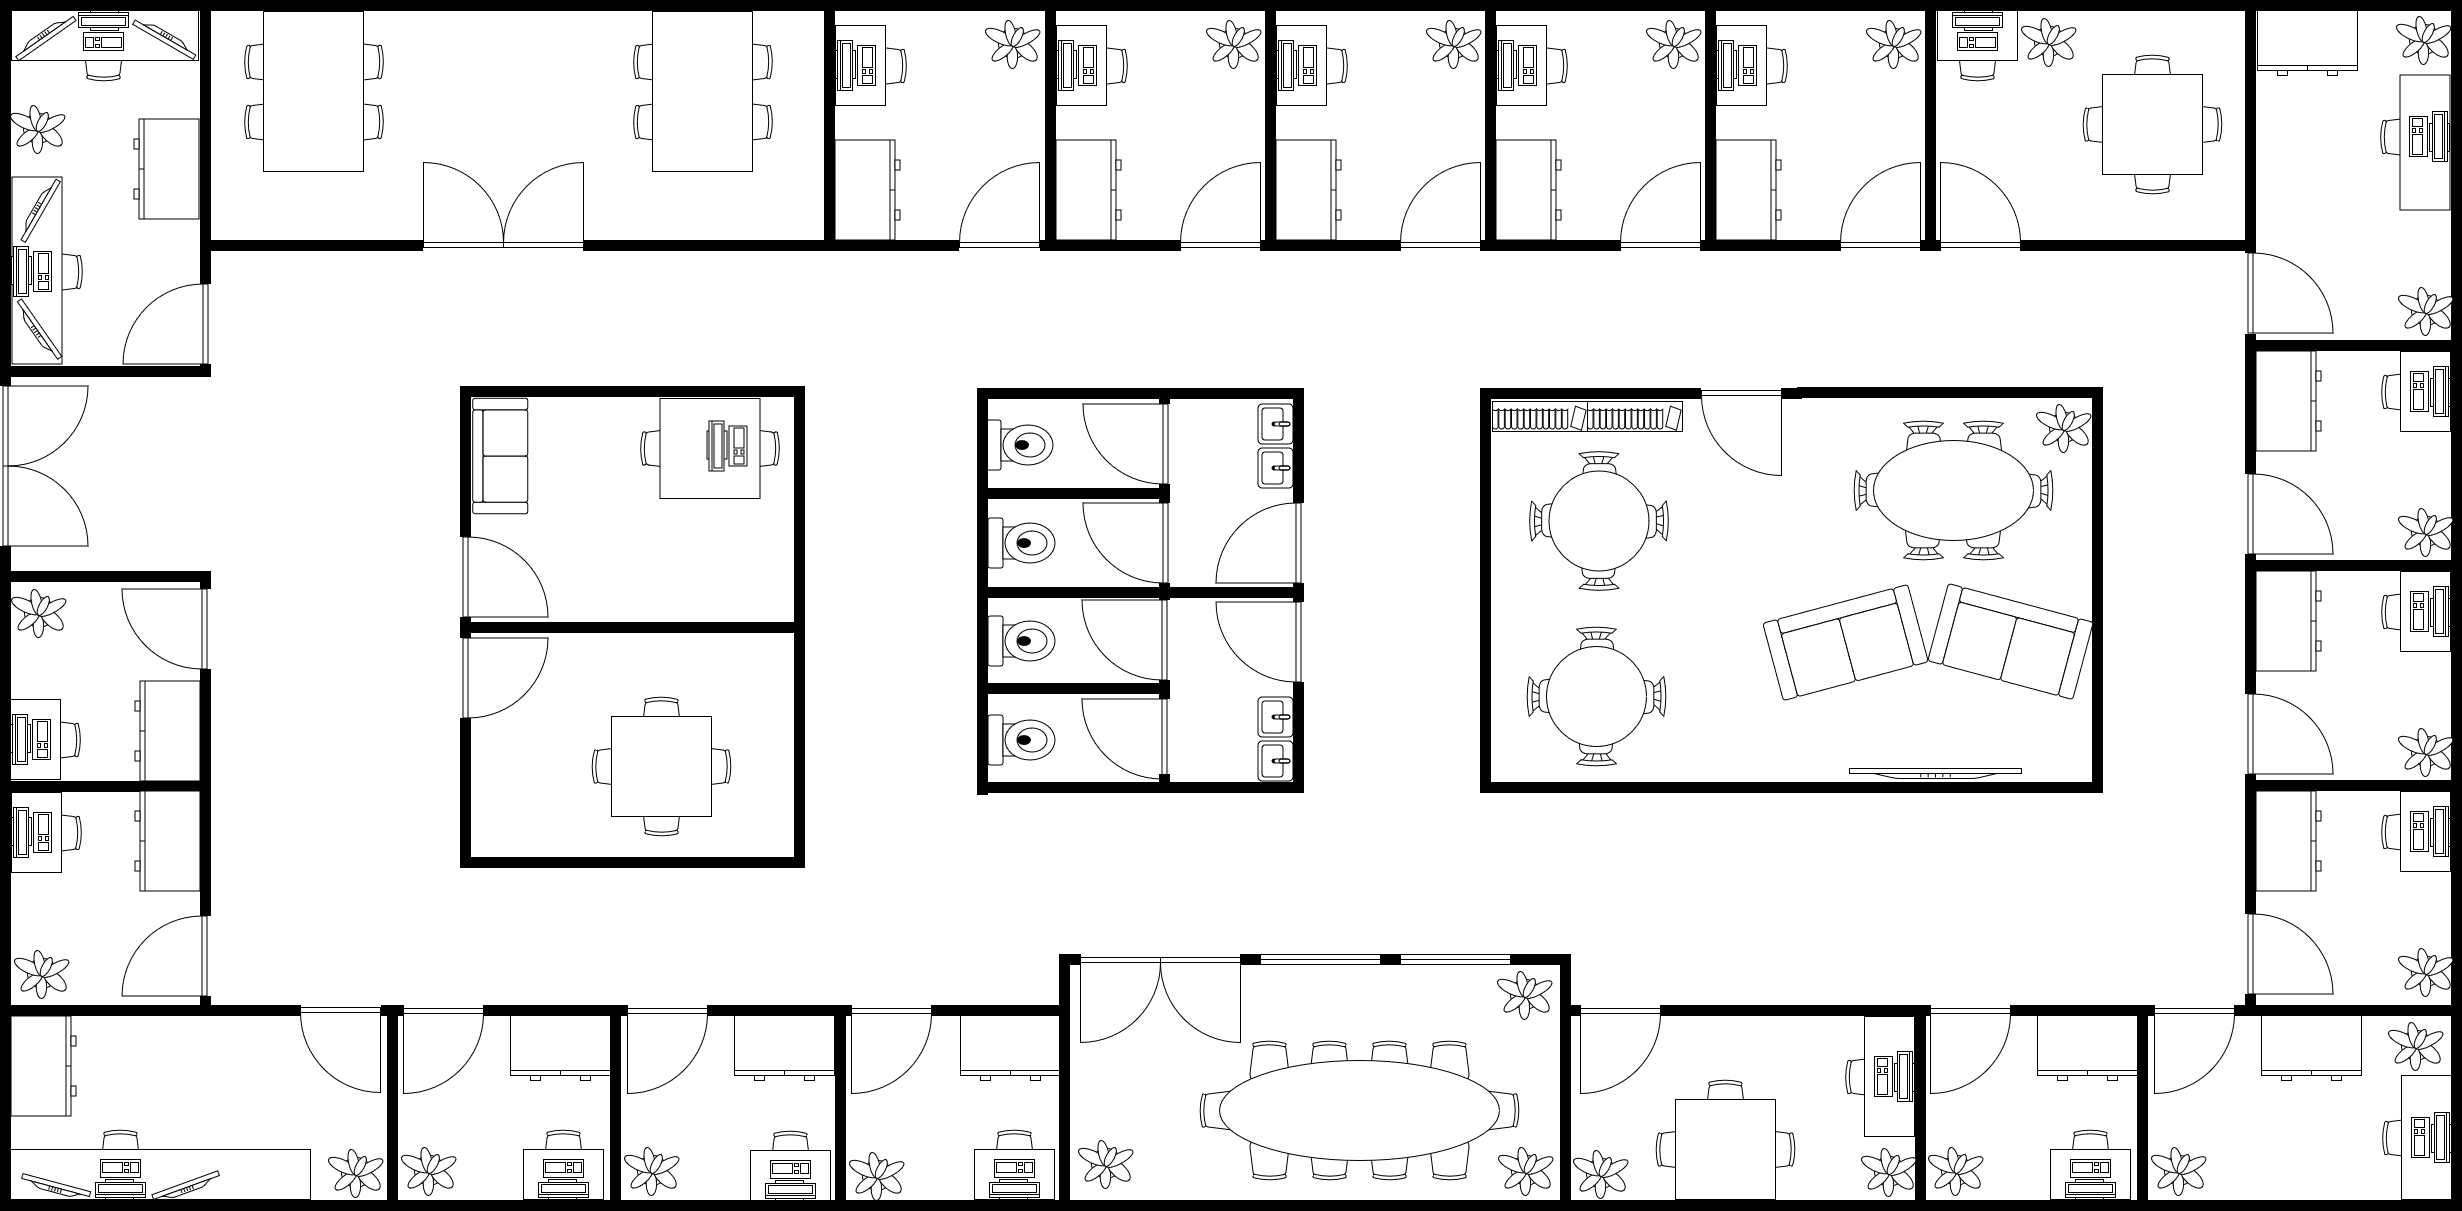
\includegraphics[width=0.9\textwidth,keepaspectratio]{planta}
		\label{fig:planta}
		\centering
		\caption{Planta das Instalações}
	\end{figure}
	
	\pagebreak
	
	\large
	\section{Análise de Mercado}
	
	\normalsize
	
	\large
	\subsection{Evolução Histórica e Previsional do Setor (Problemas e Tendências)}
	
	\normalsize
	
	Com a solução apresentada, pretendemos nos inserir no sector de software imobiliário para efeitos rurais, através da prestação de serviços (SaaS). O modelo SaaS tem vindo a crescer ao longo dos anos, com previsões para continuar esse crescimento, à medida que cada vez mais pessoas possuem um smartphone e os níveis de literacia informática aumentam. Devido a esse crescimento na procura, espera-se também um crescimento contínuo da oferta, nascendo cada vez mais empresas que utilizam esse modelo de negócio. 
	
	Um grande problema de serviços em zonas mais rurais é o acesso às mesmas, pois muitas vezes não compensa uma empresa se deslocar para essas zonas e fornecer os seus serviços.
	
	\begin{figure}[h]
		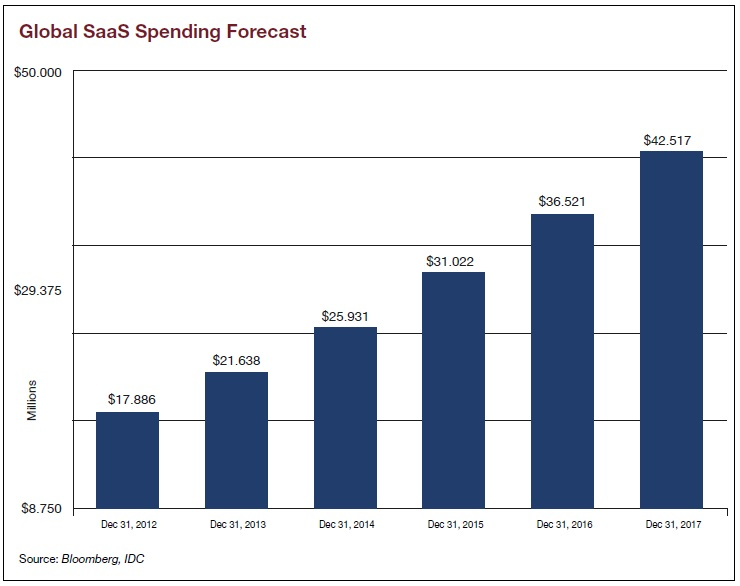
\includegraphics[width=0.6\textwidth,keepaspectratio]{crescimentoSaaS}
		\label{fig:crescimentoSaaS}
		\centering
		\caption{Crescimento do Modelo SaaS}
	\end{figure}
	
	
	
	\large
	\subsection{Enquadramento do Negócio no Setor}
	
	\normalsize
	
	O nosso negócio pretende responder a esta necessidade crescente de produtos de software no mercado imobiliário rural, procurando atingir um público que, até aos dias de hoje, não teve muita representação a esse nível, devido aos seus reduzidos conhecimentos de informática (pois muitas vezes os proprietários de terras são, por exemplo, de idade avançada e sem smartphone), algo que está de dia para dia a mudar.
	
	Usando a nossa solução de negócio o modelo SaaS, poderá, através do uso autónomo da mesma por parte dos utilizadores, alcançar todas as zonas rurais do mundo, desde que exista um acesso à Internet nas mesmas.
	
	
	\large
	\subsection{Caracterização do Mercado Alvo}
	
	\normalsize
	
	Atendendo a um pequeno estudo de mercado que efetuamos, cerca de 80\% dos indivíduos e família em primeiro e segundo grau (filhos, pais e avós) possuem pelo menos um terreno (sem construções). Para além disso, 63\% desses participantes afirmaram não conhecer todos os limites dos seus ou dos terrenos da sua família.
	
	Considerando que existem cerca de 500.000 desses conjuntos de pessoas em Portugal, podemos considerar que o número de potenciais clientes é de 63\% de 400.000, ou seja, aproximadamente 250.000. Se considerarmos toda a Europa, e usando a mesma estatística de 80\% e 63\%, temos um número de potenciais clientes de cerca de 19.000.000 (embora esse número tenha uma grande margem de erro, devido à natureza do nosso estudo de mercado). Considerando que 5\% das pessoas afetadas por esse problema seriam clientes da nossa aplicação (12.500 em Portugal, 950.000 na Europa) e que, em média, 40\% dos utilizadores do nosso serviço gastariam dinheiro com ele (5.000 em Portugal, 380.000 na Europa), e ainda considerando uma média de 30€/ano de gastos por cliente, temos, por ano, uma receita de 150.000€ em Portugal, ou 11.400.000€, na Europa.
	
	Consideramos que os clientes vão comprar o nosso serviço, pois este satisfará bem a necessidade destes guardarem um registo informático das suas posses, a um preço reduzido.
	
	
	\large
	\subsection{Análise da Concorrência}
	\subsubsection{Identificação}
	
	\normalsize
	
	\begin{center}
		\begin{tabular}{ | p{0.3\textwidth} | c | c | }
			\hline
			& Nacional & Internacional \\
			\hline
			Plano Base & BUPi & Provas de Conceito (PoC) \\
			\hline
			Plano Lifetime & BUPi & Provas de Conceito (PoC) \\
			\hline
			Plano Subscrição 1: Anúncios no Mercado & Imobiliárias & Imobiliárias \\
			\hline 
			Plano Subscrição 2: Suporte a Terrenos Cultivados & - & Croptracker \\
			\hline   
			Plano Premium & - & - \\
			\hline
		\end{tabular}
	\end{center}

	\pagebreak
	
	\large
	\subsubsection{Avaliação da Empresa com os seus Principais Concorrentes}
	\normalsize
	
	\begin{center}
		\begin{tabularx}{\linewidth}{ | c | c | X | }
			\hline
			& +/0/- & Porquê \\
			\hline
			Gama de Produtos / Serviços & + & Os concorrentes apenas oferecem soluções para um dos problemas referidos, enquanto a AquiTerrenos oferece solução para vários deles. \\
			\hline
			Qualidade dos Serviços & + & A nossa aplicação estará no topo em relação à qualidade de software. \\
			\hline
			Serviços Complementares & 0 & A AquiTerrenos terá apoio ao cliente, tal como os seus concorrentes. \\
			\hline 
			Dimensão & - & Tratando-se a AquiTerrenos de uma start-up, esta tem dimensão bastante reduzida. \\
			\hline   
			Notoriedade & - & Como a AquiTerrenos não está, de momento, no mercado, esta não tem qualquer notoriedade. \\
			\hline
			Imagem & - & Como a AquiTerrenos não está, de momento, no mercado, este não formou qualquer imagem da mesma. \\
			\hline
			Preço & + & Um dos objetivos da AquiTerrenos é fornecer planos de baixo custo e de qualidade. \\
			\hline
			Rapidez de Execução & + & Tratando-se a nossa solução de uma aplicação totalmente controlada pelo utilizador, esta é tão rápida quanto o próprio utilizador. \\
			\hline
			Garantias & + & A AquiTerrenos oferece garantias de proteção da privacidade de dados dos clientes, assim como estabilidade do serviço. \\
			\hline
		\end{tabularx}
	\end{center}
	
	
	\large
	\subsection{Fornecedores}
	
	\normalsize
	
	Tratando-se de uma empresa cujo modelo de negócio passa por uma solução SaaS, a totalidade dos fornecedores são os fornecedores dos FSE, ou seja, fornecedores de coisas como eletricidade, água e material de escritório. No entanto, há um fornecedor bastante relevante: a empresa que tratará do hosting dos servidores necessários à nossa aplicação. Esta deve oferecer garantias de funcionamento constante do mesmo, sem problemas de rapidez.
	
	\pagebreak
	
	\large
	\section{Estratégia de Marketing}
	
	\normalsize
	
	
	\large
	\subsection{Segmentação}
	
	\normalsize
	
	
	\large
	\subsection{Política do Produto/Serviço}
	
	\normalsize
	
	
	\large
	\subsection{O Preço}
	
	\normalsize
	
	
	\large
	\subsection{Distribuição}
	
	\normalsize
	
	
	\large
	\subsection{Promoção}
	
	\normalsize
	
	\pagebreak
	
	\large
	\section{Organização e Gestão}
	
	\normalsize
	
	
	\large
	\subsection{Experiência dos Promotores}
	
	\normalsize
	
	
	\large
	\subsection{Especialização Funcional da Organização}
	
	\normalsize
	
	
	\large
	\subsubsection{Organigrama}
	
	\normalsize
	
	
	\large
	\subsection{Análise da Adequação do Perfil às Funções}
	
	\normalsize
	
	
	\large
	\subsection{Processo de Decisão}
	
	\normalsize
	
	
	\large
	\subsection{Qualificações do Quadro de Recursos Humanos}
	
	\normalsize
	
	
	\large
	\subsection{Gestão de Recursos Humanos}
	
	\normalsize
	
	
	\large
	\subsection{Profissionais Externos}
	
	\normalsize
	
	\pagebreak
	
	\large
	\section{Riscos do Negócio}
	
	\normalsize
	
	
	\large
	\subsection{Análise Externa - Ameaças e Oportunidades}
	
	\normalsize
	
	
	\large
	\subsubsection{Ambiente Geral ou Macroambiente}
	
	\normalsize
	
	
	\large
	\subsubsection{Ambiente da Indústria ou Competitivo}
	
	\normalsize
	
	
	\large
	\subsubsection{Análise Interno - Forças e Fraquezas}
	
	\normalsize
	
	
	\large
	\subsection{Análise SWOT}
	
	\normalsize
	
	
	\large
	\subsection{Modelo das 5 Forças de Porter}
	
	\normalsize
	
	
	\large
	\subsubsection{Ameaça de Novas Entradas}
	
	\normalsize
	
	
	\large
	\subsubsection{Ameaça de Serviços Substitutos}
	
	\normalsize
	
	
	\large
	\subsubsection{Rivalidade Entre os Concorrentes}
	
	\normalsize
	
	
	\large
	\subsubsection{Poder Negocial dos Clientes}
	
	\normalsize
	
	
	\large
	\subsubsection{Poder Negocial dos Fornecedores}
	
	\normalsize
	
	\pagebreak
	
	\large
	\section{Plano de Implementação}
	
	\normalsize
	
	\pagebreak
	
	\large
	\section{Análise da Viabilidade Económica e Financeira}
	
	\normalsize
	
	\large
	\subsection{Pressupostos do Projeto}
	
	\normalsize
	
	
	\large
	\subsection{Investimento e Financiamento Previsionais}
	
	\normalsize
	
	
	\large
	\subsection{Proveitos e Custos Previsionais}
	
	\normalsize
	
	\pagebreak
	
	\large
	\section{Análise de Viabilidade: Cash-Flow, VAL, TIR e PayBack}
	
	\normalsize
	
	\pagebreak
	
	\large
	\section{Análise de Sensibilidade}
	
	\normalsize
	
	
	\pagebreak
	
	\large
	\section{Anexos}
	
	\normalsize
	
	
	\large
	\subsection{Demonstrações Económico-Financeiras}
	
	\normalsize
	
	
	\large
	\subsubsection{Conta Estado e Outros Enter Públicos}
	
	\normalsize
	
	
	\large
	\subsubsection{Demonstrações de Resultados Previsionais}
	
	\normalsize
	
	
	\large
	\subsubsection{Balanços Previsionais}
	
	\normalsize
	
	
	\large
	\subsection{Indicadores}
	
	\normalsize

	\pagebreak

	\listoffigures
\end{document}